\documentclass[letterpaper]{article}
\usepackage[submission]{aaai2027}
\usepackage[hyphens]{url}
\usepackage{graphicx}
\urlstyle{rm}
\def\UrlFont{\rm}
\usepackage{natbib}
\usepackage{caption}
\usepackage{booktabs}
\frenchspacing
\pdfinfo{/TemplateVersion (2027.1)}
\setcounter{secnumdepth}{0}
\title{Sensor Metadata and Axis-Aware Tokenization Govern Foundation-Model Transfer to OPM-MEG}
\author{Anonymous Authors}
\affiliations{}
\begin{document}
\maketitle

\begin{abstract}
Electrophysiological foundation models are trained almost entirely on cryogenic SQUID and EEG recordings, yet on-scalp optically pumped magnetometers (OPMs) are becoming the growth area of magnetoencephalography. We audit how one pretrained model, BrainOmni, behaves when the recording hardware changes, using only interventions on its inputs and no weight updates. Two input properties dominate. First, the categorical sensor-type tag: relabelling radial OPM magnetometers as gradiometers raises zero-shot waveform reconstruction from $0.2501$ to $0.3819$ Pearson correlation in all 21 participants of a single-axis cohort, and reproduces on native SQUID magnetometers in a single-participant control ($0.4105 \to 0.7130$). The tokenizer is therefore keyed to a discrete label that carries no waveform information. Second, channel grouping in triaxial arrays: in a complete $2\times3$ grid crossing partition type with filtering, partitioning the spatial attention by sensing axis beats a size-matched random three-way partition under identical filtering by $+0.1096$ correlation with Soft-HFC and $+0.1135$ without it, in $10/10$ participants in both regimes, while the random partition itself gains only $+0.0292$ and $+0.0269$ over a monolithic 16-query bottleneck. Pass count accounts for about one fifth of the total gain and axis-aligned grouping for the rest. The split is descriptive, a partition of the measured total rather than a causal estimate, but both components are now measured rather than assumed. Neither reconstruction gain transfers to decoding: a classical decoder over six log band powers and four temporal window means per channel outperforms the pretrained linear probe on tactile Braille classification in all eight array configurations, and under Soft-HFC its interval excludes chance while the probe's does not. We also document a window-construction shortcut that inflated an earlier evoked-detection result in this benchmark, and we exclude that task. The practical conclusions are that sensor category should be parameterized continuously rather than as a learned discrete token, that spatial query capacity should be allocated per sensing axis, and that reconstruction correlation is not a substitute for a decoding endpoint with a competitive classical baseline.
\end{abstract}

\section{Introduction}
Foundation models for electrophysiology aim at representations reusable across recording configurations and tasks. BrainOmni unifies EEG and MEG through sensor-conditioned tokenization and masked-token modeling \citep{xiao2025brainomni}. Its pretraining corpus is cryogenic: SQUID arrays mounted in a rigid dewar, 20--40\,mm from the scalp, in which gradiometers outnumber magnetometers by more than four to one. Optically pumped magnetometers invert most of these conditions. They sit roughly 5\,mm from the scalp, follow individual head shape, and in current triaxial packages place three mutually orthogonal sensing channels at one coordinate.

That makes OPM-MEG a natural stress test for the sensor-conditioning interface of such models, which is where hardware enters the computation. We hold the pretrained weights fixed and intervene only on what the model is told about its sensors: the categorical sensor-type tag, the position and orientation vectors, and the grouping of channels passed through spatial attention. The question is not whether the model can be fine-tuned onto OPM data, but which of its inputs its learned representation is actually sensitive to, and whether the resulting changes survive as decoding gains.

Our contributions are: (i) a paired, per-participant quantification of sensor-type and geometry sensitivity on two public OPM cohorts with a SQUID control; (ii) a preprocessing-matched comparison that separates axis-aware tokenization from spatial capacity, which earlier analyses of this benchmark confounded; (iii) a negative decoding result with a competitive classical baseline, showing that reconstruction gains do not propagate; and (iv) a documented evaluation shortcut that produced an apparent transfer advantage, reported so that others can avoid it.

\section{Data and Evaluation}

\subsection{Datasets}
\textbf{Single-axis OPM.} FACE-DEC, OpenNeuro ds005107 \citep{xu2024face}. We use 21 participants and the 50 channels matched across participants by rounded position and orientation metadata. The dataset documentation states that sensor coordinates were approximated from an Elekta layout for topographic display and are not measured OPM positions \citep{facedecdocs}. A shared channel set is therefore not evidence of anatomical alignment, and spatial perturbations on this cohort test the model's response to supplied metadata rather than to physical geometry.

\textbf{Triaxial OPM.} The 10 adult participants of Zenodo record 11126593 \citep{rier2024dataset}, 84 cached trials each, 155--176 retained channels, geometry in head coordinates. Retained radial and tangential subsets contain 53--60 and 102--116 channels. The task contrasts index-finger and little-finger tactile stimulation. Results apply to this adult subset, not the full developmental cohort.

\textbf{SQUID control.} Participant sub-01, run-01 of OpenNeuro ds000117 \citep{wakeman2015}, with 102 magnetometers and 204 planar gradiometers. This is a single-participant diagnostic used only to test whether the sensor-type effect is OPM-specific.

\subsection{Model, Endpoint and Interventions}
We evaluate the pretrained BrainOmni tiny configuration. Its tokenizer combines a temporal convolutional encoder with spatial cross-attention between 16 learned queries and per-channel embeddings of position, unit orientation and discrete sensor type, followed by residual vector quantization. The sequence backbone is bidirectional and trained by masked-token prediction over codebook entries, not autoregressively; we state this because the distinction bears on what the backbone can represent. Reconstruction uses the tokenizer encoder, quantizer and decoder with weights frozen.

The primary endpoint is Pearson correlation (PCC) between the reconstructed and the normalized input waveform window. This is reconstruction of the observed input, which still contains residual artifact, so a higher PCC establishes closer agreement with that target and not improved source localization, denoising or physiological validity. Participant-level scores are aggregated as saved; in the triaxial pipeline each participant's score is the mean over batch-level PCC values at batch size 16, where the final short batch carries equal weight. We retain that aggregation to match the saved results and flag trial-weighted aggregation as a reproducibility check.

Interventions on the single-axis array reassign the sensor tag from magnetometer (\texttt{MAG=1}) to gradiometer (\texttt{GRAD=2}), zero the orientation vectors, reverse them, or jointly permute position and orientation across channels, in every case leaving the waveforms untouched. All single-axis conditions share channel selection and soft homogeneous field correction (Soft-HFC), $P = I - \alpha Q_R Q_R^{\top}$ with $\alpha = 0.25$, where $Q_R$ is an orthonormal basis for the sensor-orientation subspace. Soft-HFC attenuates any component projecting onto that subspace, including neural signal, so its effect is separated from tokenization throughout.

For triaxial arrays the monolithic tokenizer passes all retained channels through one spatial bank. Axis partitioning passes the $X$, $Y$ and $Z$ groups separately through the same pretrained tokenizer and reassembles the reconstructions, giving three 16-query passes instead of one. The random three-way control splits channels into three approximately equal groups with seed 42, matching pass count but not physical grouping. All three partition types were run both without filtering and under Soft-HFC, giving a complete $2\times3$ grid in which every contrast of interest holds filtering constant.

\subsection{Statistics}
All comparisons are paired within participant. We report the mean paired difference with a percentile bootstrap confidence interval over participants (20{,}000 resamples), the number of participants in which the difference has the stated sign, and an exact two-sided sign-flip permutation $p$-value enumerating all $2^{n}$ assignments. With $n=10$ the smallest attainable $p$ is $2/2^{10} \approx 0.002$, so triaxial $p$-values at that value indicate perfect consistency rather than a precisely estimated tail. No new model inference was run for this report; every value derives from the saved per-participant records.

\begin{figure*}[t]
\centering
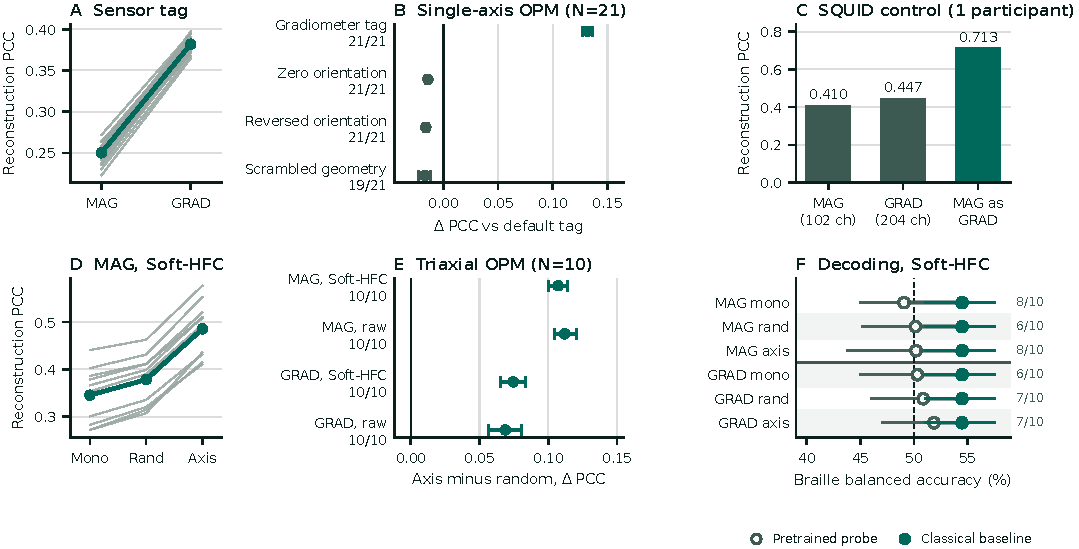
\includegraphics[width=\textwidth]{figures/transfer_overview.pdf}
\caption{Paired per-participant transfer results, read from saved per-participant records. \textbf{A}, \textbf{D}: paired trajectories, one grey line per participant, cohort mean in colour; \textbf{D} traces the monolithic, random and axis partitions under common Soft-HFC. \textbf{B}, \textbf{E}: mean paired differences with participant bootstrap 95\% confidence intervals; the count under each label is the number of participants moving in the stated direction. \textbf{B} compares each metadata intervention against the default magnetometer tag; \textbf{E} gives the capacity and grouping components of the triaxial effect, each measured within one filtering regime. \textbf{C}: single-participant SQUID diagnostic. \textbf{F}: Braille decoding, pretrained probe (open) against the classical baseline (filled), dashed line at chance; the right-hand column counts participants in which the classical decoder exceeds the probe, and the rule separates the six full-array configurations from the two channel subsets. The classical arm is invariant to partition by construction and takes four distinct values across the eight rows.}
\label{fig:overview}
\end{figure*}

\section{Results}

\subsection{A Discrete Label Dominates Reconstruction}
Table~\ref{tab:single} and Figure~\ref{fig:overview}A,B give the single-axis results. Relabelling the array from magnetometer to gradiometer, with waveforms, positions and orientations unchanged, raises reconstruction from $0.2501$ to $0.3819$, a paired difference of $+0.1318$ (95\% CI $[+0.1275, +0.1360]$), a relative increase of 52.7\%. The effect holds in 21 of 21 participants with no overlap between the two distributions, exact $p < 10^{-5}$. The SQUID control moves in the same direction and further: magnetometer-only reconstruction rises from $0.4105$ to $0.7130$ when those 102 native SQUID magnetometers are assigned the gradiometer category, a 73.7\% relative increase, on hardware the model was pretrained on.

Because the intervention changes one categorical token and nothing numerical, the result isolates a property of the learned embedding rather than of the recording. It is consistent with the gradiometer subspace having absorbed most of the MEG pretraining signal, but it does not establish that pretraining imbalance caused it; a controlled pretraining experiment would be required for that. Its practical implication is independent of the cause. A model whose reconstruction fidelity moves by half its own magnitude in response to a label that carries no waveform information has made sensor category a load-bearing free parameter at inference time.

The geometry perturbations move in the opposite direction and are small: zeroing orientations costs $-0.0142$ ($0/21$ participants improved), reversing them $-0.0161$ ($0/21$), and scrambling position and orientation jointly $-0.0171$ ($2/21$). The tokenizer does read the directional vectors, but on this cohort the discrete tag is roughly eight times more consequential than the continuous geometry. Given that FACE-DEC coordinates are approximate, we read the geometry perturbations as evidence about metadata sensitivity rather than about forward-field accuracy.

\begin{table}[t]
\centering
\small
\setlength{\tabcolsep}{4pt}
\begin{tabular}{lrr}
\toprule
Condition & PCC [95\% CI] & $\Delta$ (consist.) \\
\midrule
Default (\texttt{MAG=1}) & .2501 [.2450, .2549] & baseline \\
Gradiometer tag & .3819 [.3779, .3859] & $+.1318$ (21/21) \\
Zero orientation & .2359 [.2295, .2421] & $-.0142$ (0/21) \\
Reversed orient. & .2340 [.2274, .2402] & $-.0161$ (0/21) \\
Scrambled geometry & .2330 [.2307, .2354] & $-.0171$ (2/21) \\
\bottomrule
\end{tabular}
\caption{Waveform reconstruction on FACE-DEC (21 participants, 50 shared channels, Soft-HFC $\alpha = 0.25$). $\Delta$ is the mean paired difference against the default tag; consistency counts participants moving in that direction. Coordinates are approximate, which limits anatomical interpretation of the geometry rows.}
\label{tab:single}
\end{table}

\subsection{Axis Grouping, Separated From Capacity}
Table~\ref{tab:tri} reports the $2\times3$ grid and Figure~\ref{fig:overview}D,E the contrasts within it. Because the grid is complete, grouping and capacity separate by direct measurement rather than by assumption.

Against a size-matched random partition under identical filtering, axis partitioning gains $+0.1096$ ($[+0.1009, +0.1193]$) with Soft-HFC and $+0.1135$ ($[+0.1040, +0.1253]$) without it, in $10/10$ participants in both regimes. The random partition, which buys the same three tokenizer passes without physical grouping, gains only $+0.0292$ ($[+0.0228, +0.0349]$) and $+0.0269$ ($[+0.0205, +0.0333]$) over the monolithic baseline. Splitting the total axis-over-monolithic gain into these two measured components attributes 21.0\% to pass count and 79.0\% to orientation grouping under Soft-HFC, and 19.2\% against 80.8\% without it. The split is an algebraic partition of the total, but both components are separately measured under constant filtering, which is what earlier analyses of this benchmark lacked.

Filtering behaves as a nuisance term rather than an interaction: Soft-HFC costs $-0.0265$ on the monolithic array, $-0.0242$ on the random partition and $-0.0281$ on the axis partition, all in $0/10$ participants. Axis partitioning therefore recovers its advantage against a filter that is working against it, and the effect does not depend on which filtering regime is chosen.

Radial-only and tangential-only configurations reach $0.4944$ and $0.4446$ on channel subsets, so they are not full-array improvements. Their relevance is that discarding two thirds of the array still beats passing all of it through one 16-query bank.

\begin{table}[t]
\centering
\small
\setlength{\tabcolsep}{4pt}
\begin{tabular}{llr}
\toprule
Configuration & HFC & PCC [95\% CI] \\
\midrule
Monolithic, all channels & no & .3726 [.3405, .4048] \\
Monolithic, all channels & Soft & .3461 [.3100, .3815] \\
Random 3-way & no & .3995 [.3689, .4286] \\
Random 3-way & Soft & .3753 [.3414, .4074] \\
Axis partition & no & .5130 [.4832, .5436] \\
Axis partition & Soft & .4849 [.4500, .5197] \\
\midrule
Radial only ($Z$) & no & .4944 [.4666, .5273] \\
Tangential only ($X$, $Y$) & no & .4446 [.4111, .4773] \\
\bottomrule
\end{tabular}
\caption{Triaxial reconstruction, 10 adults, 84 trials each. The upper block is a complete $2\times3$ grid crossing partition type with filtering, so every contrast in the text compares rows with identical filtering. The lower block reconstructs channel subsets and is not comparable to the full-array rows. Intervals are percentile bootstrap over participants, recomputed here from the per-participant records with a fixed seed, so they agree with the supplement to the digits shown.}
\label{tab:tri}
\end{table}

\subsection{Reconstruction Gains Do Not Reach the Decoder}
Figure~\ref{fig:overview}F gives five-fold within-participant Braille decoding for all eight configurations. The pretrained linear probe stays at chance throughout, from 47.19\% to 50.83\%, and neither axis partitioning nor the removal of filtering moves it: the axis partition reaches 50.19\% under Soft-HFC and 47.53\% without it, having gained $+0.14$ PCC in reconstruction in both regimes.

The informative comparison is the classical baseline: six log band powers spanning 1--96\,Hz plus four temporal window means per channel, classified by $L_2$-regularized logistic regression. It reaches 52.76\% to 54.50\% and exceeds the pretrained probe in every configuration, leading in 7 or 8 of 10 participants in each. Its features depend only on the channel set and the filtering, not on how channels are grouped for the tokenizer, so the classical arm takes four distinct values across the eight rows: 53.54\% on the unfiltered full array, 54.50\% under Soft-HFC, and 53.33\% and 52.76\% on the radial and tangential subsets. That invariance is itself a control. Partitioning changes the probe by up to 3.3 points while leaving the information available to that decoder untouched, and the probe still does not reach it.

This does not settle the question. Paired tests are weak at $n=10$, most intervals cross zero, and no correction is applied across configurations. The classical interval excludes chance only on the full array under Soft-HFC, at 54.50\% $[51.03, 57.65]$; elsewhere it includes chance. So the claim is narrower than a noise-floor refutation: in one condition a classical decoder separates the classes while the probe does not, and across all eight the direction never reverses. Reconstruction fidelity and linear decodability are dissociated, since improving the first by 40\% relative did not move the second, but separating a representational failure from task difficulty would need a properly powered cohort.

One caveat is interpretive. On FACE-DEC the labels decoded under leave-one-subject-out evaluation (49.57\% default, 49.41\% remapped at a 20-participant budget) are attributes of the presented face, derived deterministically from stimulus index, not participant demographics.

\subsection{An Excluded Task, and Why}
An evoked visual-detection analysis in this benchmark previously reported scaling from 95.39\% to 99.81\% balanced accuracy and a $+4.38$ percentage point advantage of the full model over a tokenizer-only control. We exclude it. The two classes are built differently: the active class takes 128 consecutive samples of the post-stimulus window, whereas the baseline class writes one 64-sample pre-stimulus segment twice into the same 128-sample slot. The baseline class is therefore exactly periodic at lag 64 and the active class is not, and any decoder sensitive to that autocorrelation separates the classes without using evoked physiology. The same construction underlies the detection rows of the SQUID control, which we also exclude.

The failure mode is general. A positive control built to equalize window position can still fail to equalize window construction, and a model with more capacity to detect the artifact will appear to transfer better. Equal-duration windows drawn by an identical procedure, trial-grouped splits and a classical baseline on the same features are the minimum before such a task supports a transfer claim.

\section{Discussion and Limitations}
Two design implications follow. First, sensor category should not be a learned discrete token when the model is expected to meet hardware absent from pretraining. A continuous parameterization of sensing geometry, such as stand-off distance and baseline length, would let a new sensor occupy its own place instead of borrowing a category, and is testable against the categorical baseline. The categorical interface is where a 52.7\% change hides behind an integer.

Second, fixed spatial query capacity should be allocated per sensing axis in multi-axis arrays. The matched comparison shows that adding passes alone recovers little, and the axis partition retains the complete array. It is a pure inference-time reorganization and requires no retraining.

The limits are real. We evaluate one pretrained model on two small OPM cohorts with a single-participant SQUID diagnostic, so no harmonized cross-hardware estimate follows. FACE-DEC coordinates are approximate. Reconstruction against processed input can reward preserving non-neural structure. The capacity decomposition rests on a complete $2\times3$ grid rather than an additivity assumption, but uses a single random-partition seed and gives the monolithic tokenizer no matched token budget, so the grouping component is an upper bound. We used saved per-participant results rather than replaying raw data, so provenance is asserted at the level of code, hashes and saved outputs.

\section{Conclusion}
Transfer here is governed less by the waveforms than by two interface choices. A categorical sensor tag carrying no signal moves reconstruction by half its own magnitude, in every participant and on native SQUID hardware too. Axis-aware query allocation recovers a comparable amount in triaxial arrays, and a factorial grid separates that gain into a small pass-count component and a larger one only axis-aligned grouping delivers. Neither reaches a decoder built from band powers and window means. Continuous sensor parameterization, per-axis query allocation, and decoding endpoints with competitive classical baselines are what we would fix before claiming cross-hardware generalization.

\bibliographystyle{aaai2027}
\bibliography{references}
\end{document}
